\documentclass[hyperref={xetex}]{beamer}
\title{Einführung in Sage - Einheit 1}
\subtitle{Organisatorisches, Was ist Sage?, Basis}
\mode<article>
{
  \usepackage{fullpage}
  \usepackage{pgf}
  \usepackage[xetex]{hyperref}
  \setjobnamebeamerversion{beamer}
}

\mode<presentation>
{
  %\usetheme{Frankfurt}
 %\usetheme{My}
  \usetheme{Madrid}
  % or ...
%\usecolortheme{seagull}
  %\setbeamercovered{transparent}
  %\setbeamercovered{dynamic}
  % or whatever (possibly just delete it)
}
\usenavigationsymbolstemplate{}
\usefonttheme{structurebold}
\usepackage{multimedia}
%\usepackage{tikz}
\usepackage{fontspec,xunicode,xltxtra}

%\usepackage{polyglossia}
%\setdefaultlanguage[spelling=new, latesthyphen=true]{german}
%\setsansfont{DejaVu Sans}
%\setsansfont{Verdana}
%\setsansfont{Arial}
%\setromanfont{Linux Libertine O}
%\setsansfont{Linux Biolinum O}

\setbeamertemplate{footline}
{
\leavevmode
%\hbox{\begin{beamercolorbox}[wd=.5\paperwidth,ht=2.5ex,dp=1.125ex,
%leftskip=.3cm plus1fill,rightskip=.3cm]{author in head/foot}%
%    \usebeamerfont{author in head/foot}\insertshortauthor
%  \end{beamercolorbox}%
%  \begin{beamercolorbox}[wd=.5\paperwidth,ht=2.5ex,dp=1.125ex,leftskip=.3cm,
%rightskip=.3cm plus1fil]{title in head/foot}%
%    \usebeamerfont{title in head/foot}\insertshorttitle\hfill

\hfill\insertframenumber  \hspace{3pt}

%\inserttotalframenumber
%\hspace*{2ex}
%  \end{beamercolorbox}}%
  \vskip3pt%
}

\usepackage[ngerman]{babel}
\selectlanguage{ngerman}

%
% math/symbols
%
\usepackage{amssymb}
\usepackage{amsthm}
% \usepackage{latexsym}
\usepackage{amsmath}
%\usepackage{amsxtra} %Weitere Extrasymbole
%\usepackage{empheq} %Gleichungen hervorheben
%\usepackage{bm}
 %\bm{A} Boldface im Mathemodus

\usepackage{cellspace}
\setlength{\cellspacetoplimit}{2pt}
\setlength{\cellspacebottomlimit}{2pt}

%%%%%%%%%%%%%%%%%% Fuer Frames [fragile]-Option verwenden!
%Programm-Listing
%%%%%%%%%%%%%%%%%%
%Listingsumgebung fuer verbatim
%Grauhinterlegeter Text
%Automatischer Zeilenumbruch ist aktiviert
\usepackage{listings}
\definecolor{lgray}{gray}{0.80}
%\lstset{backgroundcolor=\color{lgray}, frame=single, basicstyle=\ttfamily, breaklines=true}
\lstnewenvironment{sage}{\lstset{backgroundcolor=\color{lgray},language=Python, emphstyle=\color{red}, frame=single, basicstyle=\ttfamily, breaklines=true,mathescape =true,escapechar=§}}{}


\usepackage{mydef}
%\usepackage{cmap} % you can search in the pdf for umlauts and ligatures
\usepackage{colonequals} %corrects the definition-symbols \colonequals (besides others)
\title{Einführung in Sage}
%
%\subtitle{Disputation} % (optional)

\author{Jochen Schulz}
% - Use the \inst{?} command only if the authors have different
%   affiliation.

\institute{Georg-August Universit\"at G\"ottingen \pgfimage[height=0.5cm]{../figures/unilogo3}}
% - Use the \inst command only if there are several affiliations.
% - Keep it simple, no one is interested in your street address.

\date{\today}

\subject{Sage}
% This is only inserted into the PDF information catalog. Can be left
% out. 

% If you have a file called "university-logo-filename.xxx", where xxx
% is a graphic format that can be processed by latex or pdflatex,
% resp., then you can add a logo as follows:

%\logo{\pgfimage[height=0.5cm]{figures/unilogo3}}


% Delete this, if you do not want the table of contents to pop up at
% the beginning of each subsection:

\AtBeginSection[]
{
  \begin{frame}<beamer>
    \frametitle{Aufbau}
    \tableofcontents[currentsection,currentsubsection]
  \end{frame}
}

\AtBeginSubsection[]
{
  \begin{frame}<beamer>
    \frametitle{Aufbau}
    \tableofcontents[currentsection,currentsubsection]
  \end{frame}
}



%%%%%%%%%%%%%%%%%%%
%Neue Definitionen
%%%%%%%%%%%%%%%%%%%

%Newcommands
\newcommand{\Fun}[1]{\mathcal{#1}}      %Mathcal fuer Funktoren
\newcommand{\field}[1]{\mathbb{#1}}     %Grundkoerper ?? in mathds

\newcommand{\A}{\field{A}}              %Affines A
\newcommand{\C}{\field{C}}              %Complexes C
\newcommand{\Fp}{\field{F}_{\!p}}       %Endlicher Koerper mit p Elementen
\newcommand{\Fq}{\field{F}_{\!q}}       %Endlicher Koerper mit q Elementen
\newcommand{\Ga}{\field{G}_{a}}         %Add Gruppenschema
\newcommand{\K}{\field{K}}              %Generischer Koerper 
\newcommand{\N}{\field{N}}              %Nat Zahlen
\newcommand{\Pj}{\field{P}}             %Projektives P
\newcommand{\R}{\field{R}} 		%Reelle Zahlen
\newcommand{\Q}{\field{Q}}              %Rationale Zahlen  
\newcommand{\Qt}{\field{H}}             %Quaternionen 
\newcommand{\V}{\field{V}}              %Vektorbuendel V
\newcommand{\Z}{\field{Z}}              %Ganze Zahlen

\newcommand{\fdg}{\;|\;}                 %fuer die gilt

%Operatoren
\DeclareMathOperator{\Abb}{Abb}
%\usepackage{sagetex}

\begin{document}
\lstset{basicstyle={\lstbasicfont\footnotesize}}


\begin{document}
\titlepage

\begin{frame}{Aufbau}
    \tableofcontents
\end{frame}

%%%%%%%%%%%%%%%%%%%%%%%%%%%%%%%%%%%%%%
\section*{Organisatorisches}
%%%%%%%%%%%%%%%%%%%%%%%%%%%%%%%%%%%%%

\begin{frame}{Organisatorisches}
\begin{itemize}
\item Anmeldung über StudIP \\
      \url{https://www.studip.uni-goettingen.de/}

{\color{blue}{Einführung in Sage (Mathematische Anwendersysteme) (WS 2013/2014)}}
\item Aufgabenblätter, Musterlösungen und Vorlesungsworksheets: \url{https://sage.math.uni-goettingen.de} (Studenten-Account).
\item Vorlesungsfolien, Zusammenfassungen und sonstige Dokumente: StudIP. 
\pause
\begin{block}{Dozent}
Jochen Schulz\\
NAM, Zimmer 04 (Erdgescho{\ss})\\
Telefon: 39-4525
Email: \href{mailto:schulz@math.uni-goettingen.de}{\texttt{schulz@math.uni-goettingen.de}}\\
XMPP: \url{jschulz1@jabber.gwdg.de}\\

\end{block}
\end{itemize}
\end{frame}

\begin{frame}{Starten des Programms}
\textbf{Vor.:} \alert{Stud.It-Account} nötig. \\
\textbf{Intranet/Wiki} (\url{https://wiki.math.uni-goettingen.de})
\begin{itemize}
\item Sage ist in Version 5.11 installiert
\item Sage nutzen: 
\begin{itemize}
\item Über \url{https://sage.math.uni-goettingen.de}. Login mit Studentendaten.
\item im Menu unter Education: \texttt{sagenotebook} startet (lokale) gui.\\
\item im Terminal: \texttt{sage}
\item Remote per \alert{x2goclient}
auf \texttt{login.math.uni-goettingen.de} oder auf die Compute-Server \\
(siehe auch \texttt{https://wiki.math.uni-goettingen.de/wiki/ComputeServer})
\end{itemize}
\end{itemize}
\end{frame}

\begin{frame}{Ablauf der Veranstaltung}
\begin{itemize}
\item Blockveranstaltung vom  31.3-11.4.2014
\item \alert{Vorlesung:} 9:15 Uhr bis ca. 11 Uhr
\item \alert{Übungsbetrieb:}
\begin{itemize}
\item 1 Übungszettel/Tag.
\item Klausurzulassung: 3 beliebige markierte Aufgaben/Woche testieren lassen (per Stern markiert)
\item Alternativ: Projektarbeit durchführen (Projekte auf dem sage-server)
\end{itemize}
\item \alert{Praktikum:} von 11:00 bis 17:00 Uhr Computerräume im Keller des MI (Multimediaraum).
\item \alert{Klausur 1:} 17.4.2014; 10:00 - 11:30; HS1/Maximum.
\item \alert{Klausur 2:} 26.4.2014; 10:00 - 11:30; HS1.
\end{itemize}
\end{frame}

\begin{frame}{Inhalt der Vorlesung}
\alert{Ziel:} Wiederholung des Stoffs Diff 1 und AGLA 1 mittels der Methoden der Computeralgebra und der numerischen Rechnung.
\begin{description}
 \item[1. Tag] Organisatorisches, Aufbau von Sage, Streifzug durch Sage
\item [2. Tag] Grundlagen, Symbolisches Rechnen, Gleichungen
\item [3. Tag] Mengen, Zahlen
\item [4. Tag] Matrizen, Vektorräume, Funktionen
\item [5. Tag] Datencontainer, Lineare Abbildungen, Eigenwert und Eigenvektoren
\item [6. Tag] Folgen, Reihen, Potenzreihen, Vertiefung Schleifen
\item [7. Tag] Funktionen, Grenzwerte, Funktionenfolgen, Grafiken
\item [8. Tag] Differentation, Taylorsche Formel, Integration
\item [9. Tag] Strings, interaktive Grafiken, GeoGebra, Komplexe Beispiele
\item [10. Tag] Fragestunde
\end{description}
\end{frame}

\begin{frame}{Aufbau}
\tableofcontents
\end{frame}



%%%%%%%%%%%%%%%%%%%%%%%%%%%%%%
\section{Was ist Sage?}
%%%%%%%%%%%%%%%%%%%%%%%%%%%%%%%%%

\begin{frame}{Mathematik-Software}

\begin{block}{Computeralgebra (CAS)}
\alert{exakte} Berechnungen von mathematischen Objekten
\end{block}
\bigskip

\begin{block}{Mathematische Objekte} 
Natürliche Zahlen, reelle Zahlen, Polynome, Funktionen,
Gruppen, Ringe, \ldots
\end{block}

\begin{block}{Numerischen Berechnungen}
\alert{näherungsweise} Berechnung von mathematischen Objekten. Im Computer 
{\color{blue}Gleitpunktdarstellung} genannt.
\end{block}


\begin{block}{Computeralgebra != Numerische Berechnung}
\begin{tabular}{ll}
 Mathematische Objekte & $\pi$, $\sqrt{2}$\\
 Gleitpunktdarstellung (8 Stellen)& $3.1415927$, $1.4142136$
\end{tabular}
\end{block}
\end{frame}

\begin{frame}{Mathematik-Software (Auswahl)}
\begin{small}
\begin{block}{}
\begin{tabular}{ll}
\alert{Sage} & Mathematik-Software; Symbolisch und numerisch (GPL)\\
\alert{Mathematica} &einer der Grossen CAS (kommerziell)\\
 \alert{Maple} &einer der Grossen CAS (kommerziell)\\
\alert{Matlab} &Für numerische Rechnungen (inkl. Mupad,kommerziell)\\
\alert{Octave} &Für numerische Rechnungen (GPL)\\
 \alert{Maxima} & GPL, von Sage benutzt\\
\alert{Magma} & Algebra, Zahlentheorie, Geometrie (kommerziell)\\
 \alert{SymPy} &Phython-Bibliotheken; als CAS-Verwendbar (GPL)\\
 \alert{SymbolicC++} &Bibliotheken zur CA in C++ (GPL)
\end{tabular}

\medskip
Überblick:\\{\scriptsize
\url{http://en.wikipedia.org/wiki/Mathematical_software} }
\end{block}

%\alert{Spezialanwendungen}: & Cadabra (Körpertheorie)\\
%& PARI/GP (Zahlentheorie, Teil von Sage)\\
%& GAP (Gruppentheorie, Teil von Sage) \\
%& Macaulay (Algebraische Geometrie)\\
%& Singular (Algebraische Geometrie, Teil von Sage)
%\end{tabular}
\end{small}
\end{frame}

\begin{frame}{Sage}
\begin{itemize}
\item Ein Open-source (GPL) Mathematik Software System
\item Verfügbar seit 24 Februar 2005
\item Alternative zu den 4 M's: Magma, Maple, Mathematica, Matlab
\item Basiert auf Python
\item Objektorientiert
\item Besitzt Frontends für viele externe Software 
\item (Haupt-)Interface im Browser
\end{itemize}
\end{frame}


\begin{frame}{}
von Joachim Neubüser (Gründer von GAP):
 \begin{small}
\begin{quote}
    \alert{You can read (a) Theorem and its proof [. . . ] and then
    you can use (this) Theorem for the rest of your life free of
    charge, but for many computer algebra systems license fees
    have to be paid regularly [. . . ]}.  

With this situation \alert{two of the most basic rules of conduct in
mathematics are violated: in mathematics information is
passed on free of charge and everything is laid open for
checking}. 

Not applying these rules to computer algebra
systems that are made for mathematical research [. . . ]
means moving in a most undesirable direction. 

Most important: can we expect somebody to believe a result of a
program that he is not allowed to see?  
\end{quote}
 \end{small}

\end{frame}




\begin{frame}[fragile]{Sage - Stärken und Schwächen}
\alert{Stärken}
\begin{itemize}
\item Vereinigung von vielen anderen CAS und Libraries unter einer einheitlichen Oberfläche (Maxima, Pari,
GAP, R, Magma, ..., ) und damit flexibel.
\item Durch Python angebunden an eine mächtige Skriptsprache
\item geeignet für Prototyping
%\item interaktiver Quellcode-Debugger
\item umfangreiches Hilfesystem
%\item Einfaches Einbinden von C/C++ Routinen (dynamische Module)
\item Viele freie (Unterrichts-)materialien im Internet 
\item Source Code offen und gut dokumentiert (Peer Review)
\item Browserinterface erlaubt leichten Einstieg.
\end{itemize}
\pause
\alert{Schwächen}
\begin{itemize}
\item Befehlsumfang insgesamt wahrscheinlich nicht so leistungsfähig/ausgefeilt wie bei Maple, Mathematica oder Matlab.
\item Es fehlt eine gute eigenständige Entwicklungsumgebung\\(Python IDEs sind allerdings nutzbar. Alternative zum Webinterface: \alert{Cantor})
\item Performance i.a. nicht gut, aber leicht verbesserbar (Cython)
\end{itemize}
\end{frame}

%\begin{frame}{Struktur von Sage}
%\begin{center}
%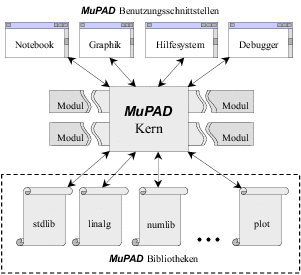
\includegraphics[width=6cm]{figures/figures/components.png}
%\end{center}
%\end{frame}


%\begin{frame}{Literatur}
%\begin{itemize}
%\end{itemize}
%\end{frame}

%%%%%%%%%%%%%%%%%%%%%%%%%%%%%%%%%%
%\section{Streifzug durch Sage}
%%%%%%%%%%%%%%%%%%%%%%%%%%%%%%%%%


%\begin{frame}[fragile]{Sage als Taschenrechner}
%Hier einige Beispiele: 
%\begin{sagecommandline}
%sage: 3+4*10+12 
%\end{sagecommandline}
%\begin{sagecommandline}
%sage: sin(pi) 
%\end{sagecommandline}
%\begin{sagecommandline}
%sage: float(pi)
%\end{sagecommandline}
%\begin{sagecommandline}
%sage: float(sqrt(2))
%\end{sagecommandline}
%\end{frame}


%%%%%%%%%%%%%%%%%%%%%%%%%%%%%%%
\subsection{Grundlagen (Sage/Python)}
%%%%%%%%%%%%%%%%%%%%%%%%%%%%%%%%%%
\begin{frame}[fragile]{Sage}
\begin{center}
\url{https://sage.math.uni-goettingen.de/home/pub/8/}
\end{center}
\end{frame}

%%%%%%%%%%%%%%%%%%%%%%%%%%%%%%%
\subsection{Eine Kurvendiskussion}
%%%%%%%%%%%%%%%%%%%%%%%%%%%%%%%%%%

\begin{frame}[fragile]{Sage}
\begin{center}
\url{https://sage.math.uni-goettingen.de/home/pub/2/}
\end{center}
\end{frame}


%
%% -> sage.math.uni-goettingen.de
%\begin{frame}[fragile]{Kurvendiskussion I}
%Betrachte die durch die reelle Zahl $a$ parametrisierte Funktionenschar:
%\[ 
%f: x \quad \mapsto \quad \frac{2x^2-20x+42}{x-1}+a, \quad
%a \in \mathbb{R} 
%\]
%
%\begin{itemize}
%\item Eingabe der Funktion
%\begin{sagecommandline}
%sage: a=var('a')
%sage: f(x) = (2*x^2-20*x +42)/(x-1)+a
%\end{sagecommandline}
%\begin{sageout}
%  x |--> a + 2*(x^2 - 10*x + 21)/(x - 1)
%\end{sageout}
%\end{itemize}
%\end{frame}
%
%\begin{frame}[fragile]{Kurvendiskussion II}
%\begin{itemize}
%\item Pol ?
%\begin{sagecommandline}
%sage: f.limit(x=1, dir='minus')
%\end{sagecommandline}
%\begin{sagecommandline}
%sage: f.limit(x=1, dir='plus') 
%\end{sagecommandline}
%%\item Umformen
%%\begin{sagecommandline}
%%f.full_simplify()
%%\end{sagecommandline}
%%\begin{sageout}
%%x |--> ((a - 20)*x + 2*x^2 - a + 42)/(x - 1)
%%\end{sageout}
%\end{itemize}
%\end{frame}
%
%\begin{frame}[fragile]{Kurvendiskussion III}
%\begin{itemize}
%\item Nullstellen
%\begin{sagecommandline}
%sage: solve(f==0,x)
%\end{sagecommandline}
%\begin{scriptsize}
%\end{scriptsize}
%\item Berechnen der Ableitung
%\begin{sagecommandline}
%sage: f.differentiate(x)
%\end{sagecommandline}
%\end{itemize}
%\end{frame}
%
%\begin{frame}[fragile]{Kurvendiskussion IV}
%\begin{itemize}
%\item Extremwerte
%\begin{sagecommandline}
%sage: maxi = solve(f.differentiate(x)==0,x); maxi 
%\end{sagecommandline}
%\begin{sageout}
%[x == -2*sqrt(3) + 1, x == 2*sqrt(3) + 1]
%\end{sageout}
%\item Lokale Minima und Maxima
%\begin{sagecommandline}
%sage: float( ((f.diff(x)).diff(x))(maxi[0].rhs()) )
%\end{sagecommandline}
%\begin{sagecommandline}
%sage: float( ((f.diff(x)).diff(x))(maxi[1].rhs()) )
%\end{sagecommandline}
%\end{itemize}
%\end{frame}
%
%\begin{frame}[fragile]{Kurvendiskussion V}
%\begin{itemize}
%\item Verhalten von $f$ für große $x$
%\begin{sagecommandline}
%sage: f.limit(x=oo); f.limit(x=-oo)
%\end{sagecommandline}
%\begin{sageout}
%x |--> +Infinity
%x |--> -Infinity
%\end{sageout}
%\item Definiere $f_{0}$, $f_{1}$, $f_{2}$
%\begin{sagecommandline}
%sage: f0 = f(x, a=0)
%sage: f1 = f(x, a=-20)
%sage: f2 = f(x, a=20);f0,f1,f2
%\end{sagecommandline}
%\begin{scriptsize}
%\begin{sageout}
%(2*(x^2 - 10*x + 21)/(x - 1), 2*(x^2 - 10*x + 21)/(x - 1) - 20, 2*(x^2 - 10*x + 21)/(x - 1) + 20)
%\end{sageout}
%\end{scriptsize}
%\end{itemize}
%\end{frame}
%

%
%\begin{frame}[fragile]{Symbolisches Rechnen I}
%\begin{itemize}
%\item Integrieren von $\int_0^\infty x^4 e^{-x} dx$
%\begin{sagecommandline}
%integrate(x^4*exp(-x),x,0,oo)
%\end{sagecommandline}
%\begin{sageout}
%  24
%\end{sageout}
%\item Stammfunktion von $\frac{1+\sin (x)}{1+\cos(x)}$
%\begin{sagecommandline}
%f(x) = (1+sin(x))/(1+cos(x))
%g = f.integrate(x)
%\end{sagecommandline}
%\begin{sageout}
%x |--> sin(x)/(cos(x) + 1) - log(cos(x) + 1)
%\end{sageout}
%\item Vereinfachen
%\begin{sagecommandline}
%g.full_simplify()
%\end{sagecommandline}
%%\begin{scriptsize}
%\begin{sageout}
%x |--> -((cos(x) + 1)*log(cos(x) + 1) - sin(x))/(cos(x) + 1)
%\end{sageout}
%%\end{scriptsize}
%\end{itemize}
%\end{frame}
%
%\begin{frame}[fragile]{Symbolisches Rechnen II}
%\begin{itemize}
%\item Faktorisieren und Ausmultiplizieren 
%\begin{sagecommandline}
%expand((x-1)*(x-2)*(x-3)*(x-4))
%\end{sagecommandline}
%\begin{sageout}
%x^4 - 10*x^3 + 35*x^2 - 50*x + 24
%\end{sageout}
%\begin{sagecommandline}
%factor(_)
%\end{sagecommandline}
%\begin{sageout}
%(x - 4)*(x - 3)*(x - 2)*(x - 1)
%\end{sageout}
%\item Sortieren eines Ausdrucks bezüglich einer Unbekannten
%\begin{sagecommandline}
%var('b,a')
%g = x^2+2*x+b*x^2+sin(x)+a*x
%g.collect(x)
%\end{sagecommandline}
%\begin{sageout}
%(b + 1)*x^2 + (a + 2)*x + sin(x)
%\end{sageout}
%\end{itemize}
%\end{frame}
%
%\begin{frame}[fragile]{Symbolisches Rechnen III}
%\begin{itemize}
%\item Partialbruchzerlegung
%\begin{sagecommandline}
%g = x^ 2/( x^ 2- 1)
%g.partial_fraction()
%\end{sagecommandline}
%\begin{sageout}
%1/2/(x - 1) - 1/2/(x + 1) + 1
%\end{sageout}
%\item Vereinfachen von Ausdrücken ($\frac{e^x -1}{e^{(1/2)x}+1}$)
%\begin{sagecommandline}
%g = (exp(x)-1)/(exp(x/2)+1)
%g.simplify_radical()
%\end{sagecommandline}
%\begin{sageout}
% e^(1/2*x) - 1
%\end{sageout}
%\end{itemize}
%\end{frame}
%
%\begin{frame}[fragile]{Zusammenfassung}
%\begin{itemize}
%\item symbolisch Integrieren: {\color{blue} \verb~integrate(f,x)~}
% \item numerisch Integrieren: {\color{blue} \verb~integrate(f,x,a,b)~}
%\item faktorisieren: {\color{blue} \verb~expand(f)~}
%\item sortieren: {\color{blue} \verb~f.collect(x)~}
%\item partialbruchzerlegung: {\color{blue} \verb~f.partial_fraction()~}
%\item vollständiges Vereinfachen: {\color{blue} \verb~f.full_simplify()~}
%\item Vereinfachen mit radicals: {\color{blue} \verb~f.radical_simplify()~}
%\end{itemize}
%\end{frame}




%%%%%%%%%%%%%%%%%%%%%%%%%%%%%%%
\subsection{Etwas AGLA}
%%%%%%%%%%%%%%%%%%%%%%%%%%%%%%%%%%
\begin{frame}[fragile]{Sage}
\begin{center}
\url{https://sage.math.uni-goettingen.de/home/pub/4/}
\end{center}
\end{frame}
%
%
%\begin{frame}{Analytische Geometrie und Lineare Algebra}
%
%Berechnen des Schnittpunkts der Ebene 
%\[ E: \vec{x}= 
%\left ( \begin{array}{c}  2 \\ 1 \\ -1 \end{array} \right) +l 
%\left ( \begin{array}{c}  1 \\ -1 \\ -1 \end{array} \right) +m
%\left ( \begin{array}{c}  -3 \\ 1 \\ 4 \end{array} \right), \quad l,m
%\in \mathbb{R}
%\]
%mit der Geraden 
%\[
%g: \vec{x}=
%\left ( \begin{array}{c}  3 \\ 0 \\ 1 \end{array} \right) +k
%\left ( \begin{array}{c}  4 \\ -1 \\ 2 \end{array} \right), \quad k \in \mathbb{R}
%\]
%\end{frame}
%
%\begin{frame}[fragile]{Grafische Darstellung}
%\begin{sagecommandline}
%var('l,m'); E1 = 2+l-3*m; E2 = 1-l+m; E3 =-1-l+4*m
%p = parametric_plot3d([E1,E2,E3],(l,-2,2),(m,-2,2), color='green', opacity=0.8)
%var('k'); g1 = 3+4*k; g2 = -k; g3 = 1+2*k
%p += parametric_plot3d( (g1,g2,g3), (k, -3, 3),thickness='3' ) 
%p.show()
%\end{sagecommandline}
%\end{frame}
%
%\begin{frame}{Grafische Darstellung}
%\begin{center}
%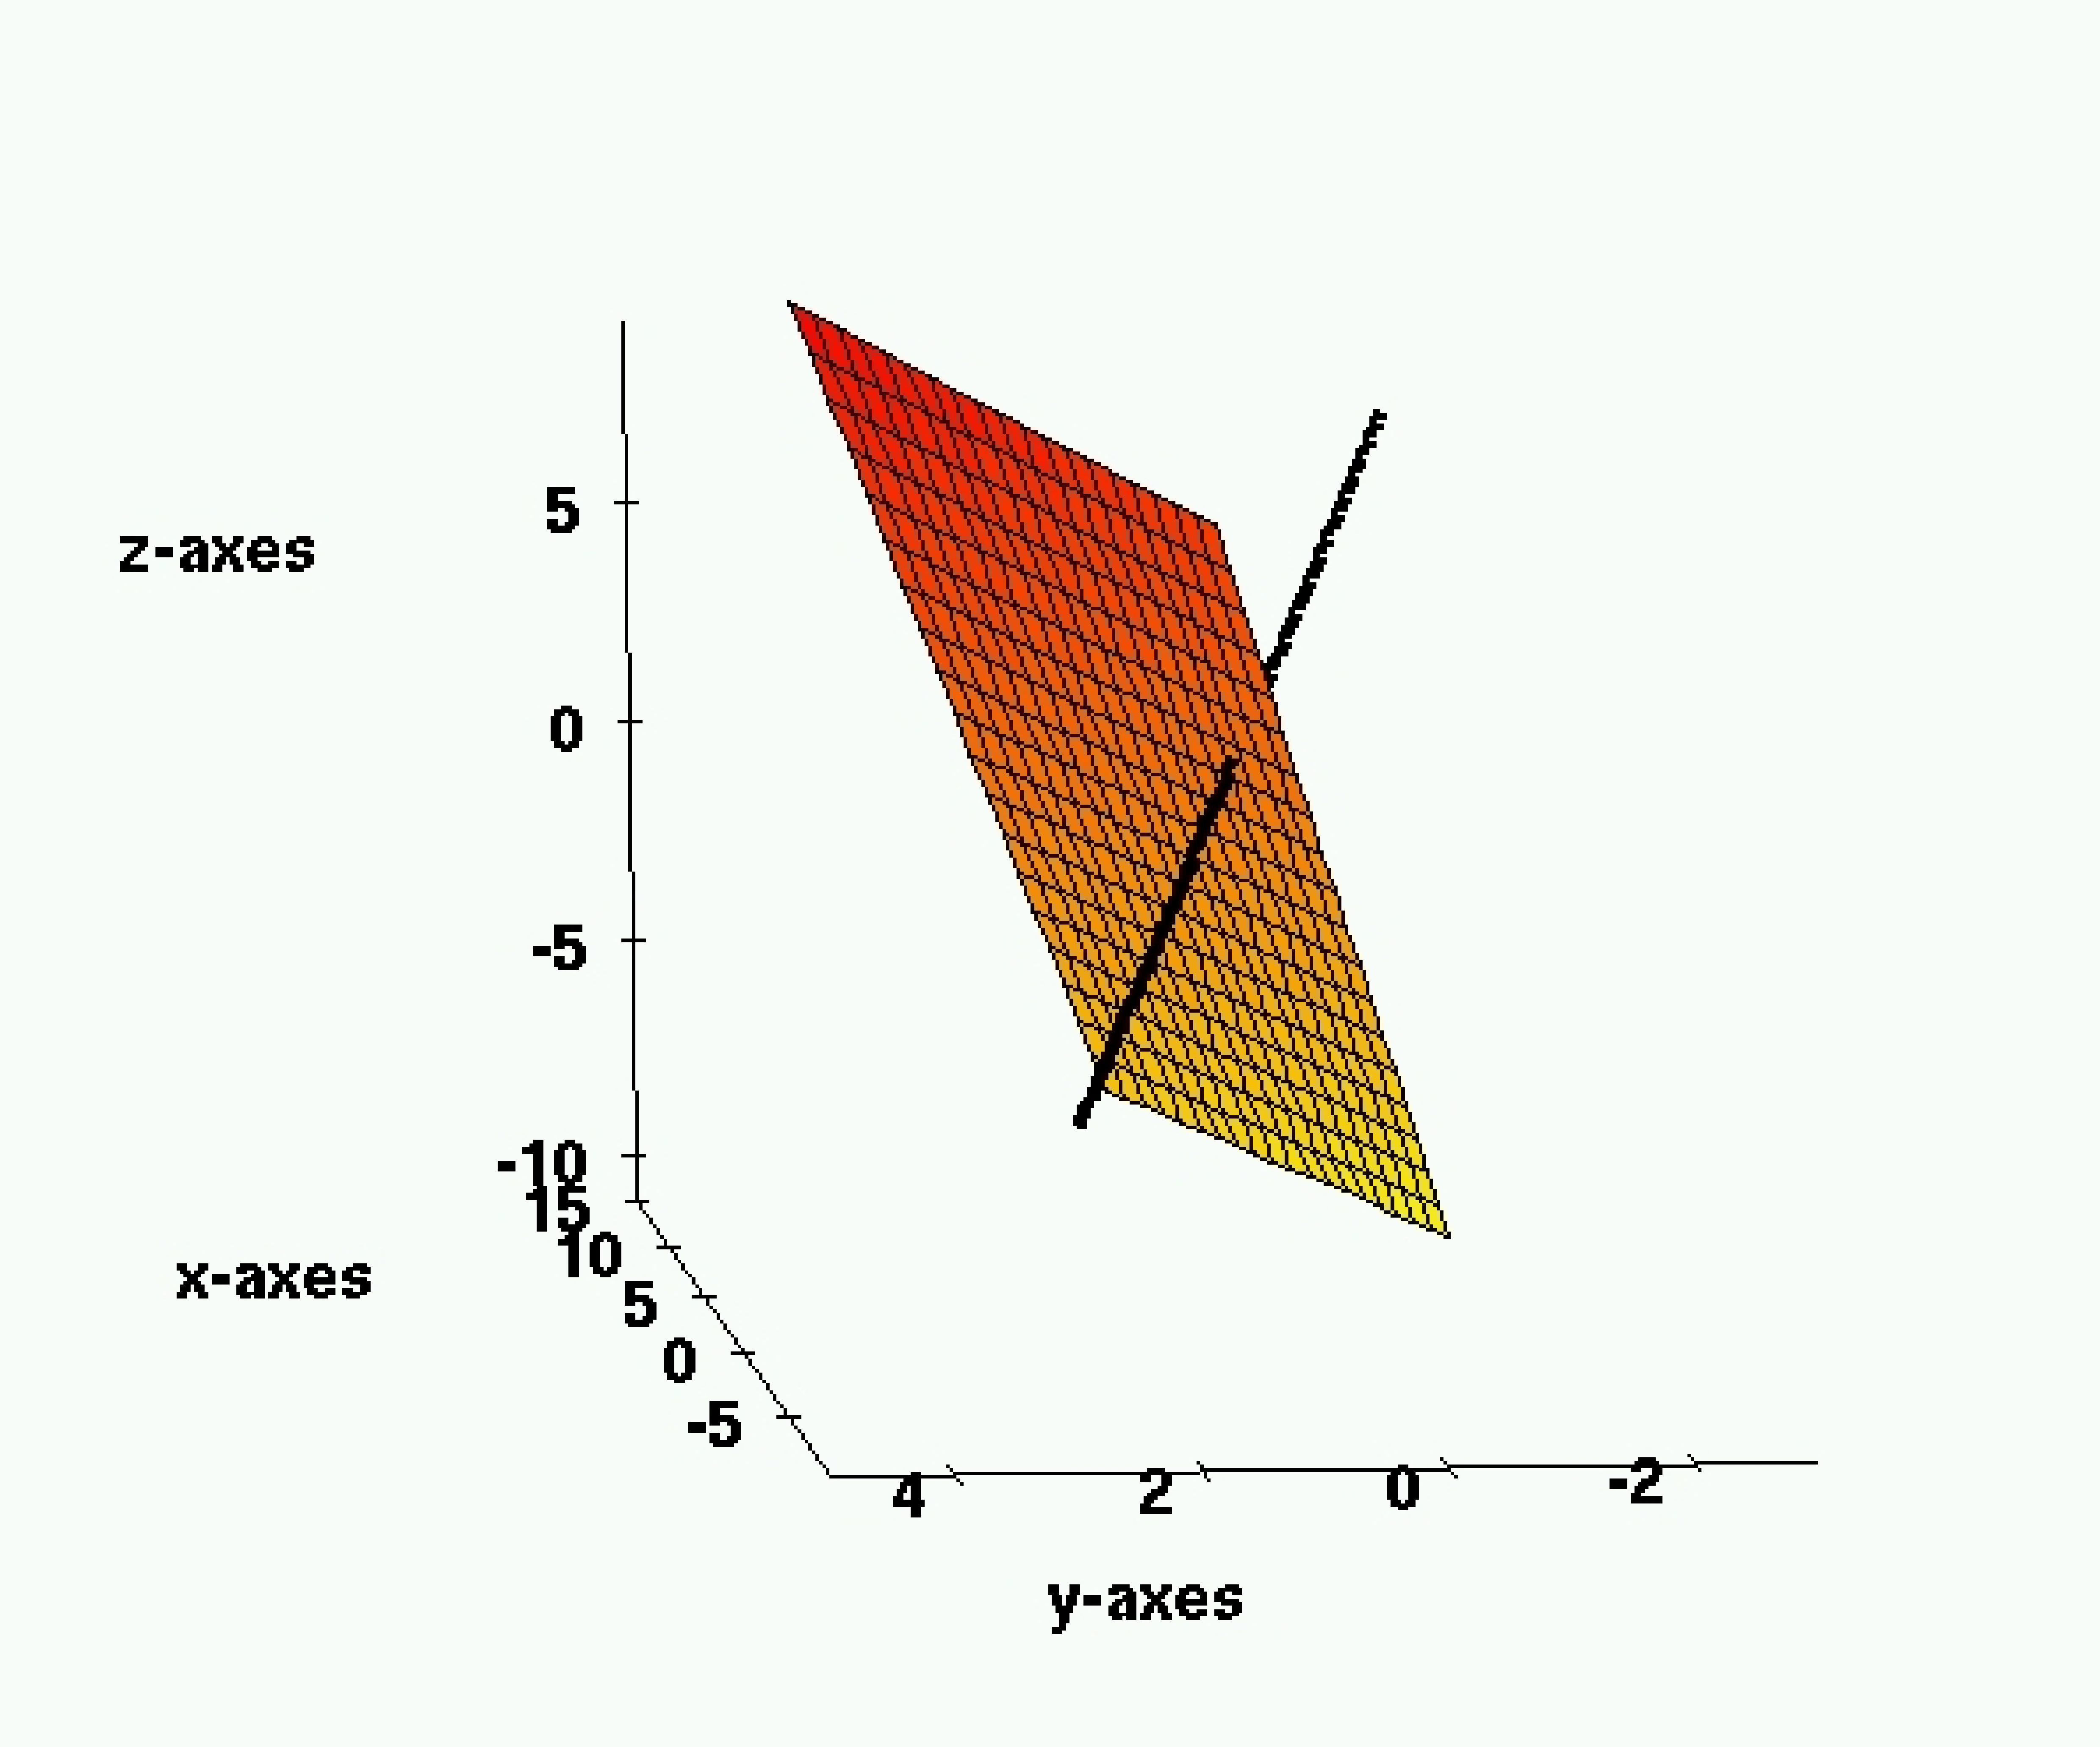
\includegraphics[width=0.7\textwidth]{figures/ebene2}
%\end{center}
%\end{frame}
%
%\begin{frame}{Analytische Lösung}
%Gleichsetzen ergibt: 
%\[ 
%\left ( \begin{array}{c}  2 \\ 1 \\ -1 \end{array} \right) +l 
%\left ( \begin{array}{c}  1 \\ -1 \\ -1 \end{array} \right) +m
%\left ( \begin{array}{c}  -3 \\ 1 \\ 4 \end{array} \right) = \left ( \begin{array}{c}  3 \\ 0 \\ 1 \end{array} \right) +k
%\left ( \begin{array}{c}  4 \\ -1 \\ 2 \end{array} \right)
%\] oder {
%\[ 
%\underbrace{\left(   
%\begin{array} {ccc} 
%1 & -3 & -4\\
%-1 & 1 & 1 \\
%-1 & 4 & -2  
%\end{array} \right)}_{\displaystyle =:A} 
%\underbrace{\left ( \begin{array}{c}  l \\ m \\ k \end{array}
%  \right)}_{\displaystyle =:L} = \underbrace{\left ( \begin{array}{c}  1 \\ -1 \\ 2
%  \end{array} \right)}_{\displaystyle =:b}
%\] }
%oder $A L=b$.
%\end{frame}
%
%\begin{frame}[fragile]{Definieren und Lösen des LGS}
%\begin{itemize}
%\item Definieren der Matrix $A$
%\begin{sagecommandline}
%A = matrix([[1,-3,-4],[-1,1,1],[-1,4,-2]]); A
%\end{sagecommandline}
%\begin{sageout}
%[ 1 -3 -4]
%[-1  1  1]
%[-1  4 -2]
%\end{sageout}
%\item Definieren des Vektors $b$
%\begin{sagecommandline}
%b = vector([1,-1,2])
%\end{sagecommandline}
%\end{itemize}
%\end{frame}
%
%\begin{frame}[fragile]
%\begin{itemize}
%\item Lösen von  $A \ L=b$
%\begin{sagecommandline}
%A.solve_right(b)
%\end{sagecommandline}
%oder 
%\begin{sagecommandline}
%A\b
%\end{sagecommandline}
%ergibt
%\begin{sageout}
%(6/5, 3/5, -2/5)
%\end{sageout}
%\item Einsetzen in die Geradengleichung
%\begin{sagecommandline}
%x_s = matrix([g1,g2,g3]).subs(k=L[2]); x_s
%\end{sagecommandline}
%\begin{sageout}
%[7/5 2/5 1/5]
%\end{sageout}
%\end{itemize}
%\end{frame}
%
%\begin{frame}[fragile]
%\begin{itemize}
%\item Matrizenoperationen
%\begin{sagecommandline}
%B = matrix([[1,0,0],[0,1,1],[1,1,1]])
%A*B; A-B; A+B
%\end{sagecommandline}
%\begin{scriptsize}
%\begin{sageout}
%[-3 -7 -7]  [ 0 -3 -4] [ 2 -3 -4]
%[ 0  2  2]  [-1  0  0] [-1  2  2]
%[-3  2  2]  [-2  3 -3] [ 0  5 -1]
%\end{sageout}
%\end{scriptsize}
%\item Berechnen der Inversen (mit Probe)
%\begin{sagecommandline}
%A^(-1), A*A^(-1)
%\end{sagecommandline}
%\begin{scriptsize}
%\begin{sageout}
%[  -2/5 -22/15   1/15]
%[  -1/5   -2/5    1/5]
%[  -1/5  -1/15  -2/15]
%
%[1 0 0]
%[0 1 0]
%[0 0 1]
%\end{sageout}
%\end{scriptsize}
%\end{itemize}
%\end{frame}
%
%\begin{frame}[fragile]{Zusammenfassung}
%\begin{itemize}
%\item Matrix eingeben: {\color{blue} \verb~matrix([ [z1s1,z1s2],[z2s1,z2s2] ])~}
% \item Vektor eingeben: {\color{blue} \verb~vector([a,b,c])~}
%\item LGS lösen: {\color{blue} \verb~A\b~}
%\item Matrixoperationen: {\color{blue} \verb~A+B,A-B,A*B~}
%\item Matrix invertieren: {\color{blue} \verb~A^(-1); A.inverse()~}
%\item Substitutieren: {\color{blue} \verb~f.subs(k=2)~}
%\end{itemize}
%\end{frame}


%%%%%%%%%%%%%%%%%%%%%%%%%%%%%%%
\subsection{Etwas Programmieren}
%%%%%%%%%%%%%%%%%%%%%%%%%%%%%%%%%%
\begin{frame}[fragile]{Sage}
\begin{center}
\url{https://sage.math.uni-goettingen.de/home/pub/5/}
\end{center}
\end{frame}


%%%%%%%%%%%%%%%%%%%%%%%%%%%%%%%
\subsection{Etwas Zahlentheorie}
%%%%%%%%%%%%%%%%%%%%%%%%%%%%%%%%%%
\begin{frame}[fragile]{Sage}
\begin{center}
\url{https://sage.math.uni-goettingen.de/home/pub/6/}
\end{center}
\end{frame}

%%%%%%%%%%%%%%%%%%%%%%%
\section{Nützliches und Hilfe}
%%%%%%%%%%%%%%%%%%%%%%%%%%%%%%%%%
\begin{frame}[fragile]{Nützliches und Hilfe}
\begin{center}
Finde man auf dem \alert{Quicksheet} (Dokument im StudIP zu finden).
%\url{https://sage.math.uni-goettingen.de/home/pub/2/}
\end{center}

\begin{block}{Anmerkung}
Programmieren lernt man am Rechner durch Übung! nehmt bitte die Möglichkeiten 
der Übung und des Praktikums wahr!
\end{block}
\end{frame}
\end{document}
